\documentclass[11pt]{amsart}
\pdfsuppressptexinfo=-1
\usepackage[margin=1.1in]{geometry}
\usepackage{amsmath,amssymb,amsthm,mathtools}
\usepackage{booktabs,enumitem}
\usepackage{xcolor}
\usepackage{tikz}
\usepackage[unicode,hidelinks]{hyperref}
\hypersetup{pdftitle={An upper bound for the connective constant of the square lattice},
  pdfauthor={Tejasvi Singh Tomar}}

\newtheorem{theorem}{Theorem}[section]
\newtheorem{lemma}[theorem]{Lemma}
\newtheorem{proposition}[theorem]{Proposition}
\newtheorem{corollary}[theorem]{Corollary}
\theoremstyle{definition}
\newtheorem{definition}[theorem]{Definition}
\theoremstyle{remark}
\newtheorem{remark}[theorem]{Remark}
\numberwithin{equation}{section}
\setlength{\emergencystretch}{2em}
\raggedbottom

% Characters of the quoted Lean source (Section 8).
\DeclareUnicodeCharacter{2200}{\ensuremath{\forall}}
\DeclareUnicodeCharacter{2203}{\ensuremath{\exists}}
\DeclareUnicodeCharacter{2115}{\ensuremath{\mathbb{N}}}
\DeclareUnicodeCharacter{211D}{\ensuremath{\mathbb{R}}}
\DeclareUnicodeCharacter{2192}{\ensuremath{\to}}
\DeclareUnicodeCharacter{2264}{\ensuremath{\le}}
\DeclareUnicodeCharacter{2227}{\ensuremath{\wedge}}
\DeclareUnicodeCharacter{2211}{\ensuremath{\sum}}
\DeclareUnicodeCharacter{03BC}{\ensuremath{\mu}}
\DeclareUnicodeCharacter{1D4DD}{\ensuremath{\mathcal{N}}}
\newcommand{\lean}[1]{\texttt{\detokenize{#1}}}
\newcommand{\LEANVERSION}{v4.35.0-rc3}
\newcommand{\MATHLIBCOMMIT}{c55e6e786f49}

\newcommand{\Z}{\mathbb{Z}}
\newcommand{\N}{\mathbb{N}}
% Certified data of the certificate (one place).
\newcommand{\Kmax}{30}
\newcommand{\LamNum}{105432502045487}
\newcommand{\LamDen}{39656386815908}
\newcommand{\LamRedNum}{105432502045487}
\newcommand{\LamRedDen}{39656386815908}
\newcommand{\LamDec}{2.658651241600}
\newcommand{\MuUB}{2.6586513}
\newcommand{\NStates}{24{,}887{,}440{,}008}
\newcommand{\NOcc}{11{,}249{,}726{,}754}
\newcommand{\NTrap}{3{,}526{,}804{,}071}
\newcommand{\NChildren}{59{,}885{,}789{,}199}
\newcommand{\NSubset}{51{,}386{,}435{,}328}
\newcommand{\NDeadA}{7{,}437{,}912{,}569}
\newcommand{\NDeadB}{1{,}640{,}728{,}376}
\newcommand{\NDeadC}{2{,}570{,}812{,}628}
\newcommand{\CouUB}{2.662342426}
% Other certificates accepted by both checkers: order 28 (k28f) in two records, orders 26 and 28 (k26f, k28e) in one.
\newcommand{\OldSuppDOI}{10.5281/zenodo.23548806}
\newcommand{\FSuppDOI}{10.5281/zenodo.23551536}
\newcommand{\FDataDOI}{10.5281/zenodo.23551538}
% Kernel-only proof of Theorem 1.1 (Section 8).
\newcommand{\KDir}{lean\_k30e}
\newcommand{\KGroup}{$16$}
\newcommand{\VsixSuppDOI}{10.5281/zenodo.23636439}
% Release slots (set at hand-off).
\newcommand{\PAPERDOI}{10.5281/zenodo.23715896}
\newcommand{\SUPPDOI}{10.5281/zenodo.23715897}
\newcommand{\DataA}{10.5281/zenodo.23574056}
\newcommand{\DataB}{10.5281/zenodo.23574058}
\newcommand{\DataC}{10.5281/zenodo.23574060}
\newcommand{\DataD}{10.5281/zenodo.23574062}
\newcommand{\DataE}{10.5281/zenodo.23574064}
\newcommand{\REPOURL}{https://github.com/tejasvi/connective-constant-bound/tree/v8}
\newcommand{\COMMITREF}{}   % set by commit.tex (outside the repository) once the release commit exists: , commit + its first 12 hex digits
\IfFileExists{commit.tex}{\input{commit.tex}}{}

\begin{document}

\title{An upper bound for the connective constant of the square lattice}
\author{Tejasvi Singh Tomar}
\renewcommand{\urladdrname}{{\itshape ORCID}}
\urladdr{\href{https://orcid.org/0000-0003-4668-3639}{https://orcid.org/0000-0003-4668-3639}}
\subjclass[2020]{82B41; 05A15, 60K35, 68Q45, 68V05, 68V20}
\keywords{self-avoiding walk, connective constant, bridges, finite automata, computer-assisted proof, formal verification}

\begin{abstract}
We prove that the connective constant $\mu$ of the square lattice $\Z^2$, the exponential growth rate of the number of $n$-step self-avoiding walks, satisfies $\mu\le\MuUB$. The previous best upper bound, $\mu\le\CouUB$, is due to Couronn\'e. Like the bounds of P\"onitz and Tittmann and of Couronn\'e, ours comes from a finite automaton that remembers a bounded part of the past of the walk. The new idea is to count bridges. Since they can all be preceded by the same infinite history, the automaton may treat as visited the unvisited cells that no infinite self-avoiding continuation can reach, and three tests on the current state and the next step recognize such cells. The bound is checked in exact integer arithmetic and proved in the Lean proof assistant.
\end{abstract}

\maketitle

\section{Introduction}\label{sec:intro}

Let $c_n$ be the number of $n$-step self-avoiding walks on the square lattice $\Z^2$ that start at the origin. Since $c_{n+m}\le c_nc_m$, the limit
\[
\mu=\lim_{n\to\infty}c_n^{1/n}
\]
exists~\cite{HaMo54}. It is called the connective constant of $\Z^2$. Its value is not known; numerical estimates give $\mu\approx2.63815853032790$~\cite{JSG16}.

Upper bounds for $\mu$ come from counting walks with a bounded memory. Alm~\cite{Alm93} proved $\mu\le2.69576$, and Noonan~\cite{Noo98} $\mu\le2.6939$. P\"onitz and Tittmann~\cite{PT00} built finite automata whose states are the last steps of the walk, with the steps that can no longer matter removed, reaching $\mu\le2.679192495$. Couronn\'e~\cite{Cou25} added several simplification rules to the automaton of P\"onitz and Tittmann and, considering loops of length up to $26$, obtained $\mu\le\CouUB$. This was the best upper bound so far. Lower bounds come from counting irreducible bridges; in this way Jensen~\cite{Jen04} obtained $\mu>2.625622$. On the hexagonal lattice the connective constant is known to be exactly $\sqrt{2+\sqrt2}$~\cite{DCS12}.

\begin{theorem}\label{thm:main}
The connective constant of the square lattice satisfies
\[
\mu\le\frac{\LamRedNum}{\LamRedDen}=\LamDec\ldots<\MuUB.
\]
\end{theorem}

Our automaton reads bridges instead of walks. This loses nothing, because for the number $b_n$ of $n$-step bridges that start at the origin the Hammersley--Welsh theorem~\cite{HW62} gives $\mu=\lim b_n^{1/n}$. Here a self-avoiding walk is a bridge if its first cell lies strictly to the left of all its other cells and its last cell lies in its rightmost column. A bridge that starts at the origin, preceded by the cells $(x,0)$ with $x<0$ and followed by translates of itself, each starting where the previous one ends, forms a two-sided infinite self-avoiding path. We give every bridge this half-line as its history. The automaton may then treat as visited every cell that the walk has not visited but that no two-sided infinite self-avoiding path extending the history and the walk so far can visit, since the walk will never visit it. We call such cells dead.

Figure~\ref{fig:dead} shows how dead cells arise. The state there is a path of $13$ cells ending at the origin, which is the current position; the next step goes to the cell $t$. Each cell marked a has three of its four neighbours in the state, so a path that entered it could not leave it. The cell marked b is enclosed by the state and~$t$. The cell marked c is connected to infinity only through the cell $w$; without $w$ it is cut off both from infinity and from the neighbours of~$t$ outside the state. These are the three tests of Definition~\ref{def:dead}. Section~\ref{sec:sound} shows that the cells these tests find are dead, although they need not find every dead cell. In general a state is a set of cells, written as a lattice path ending at the current position, each of which is visited or dead. Our construction also uses simplification rules of~\cite{Cou25} that put unvisited cells into a state; in our certificate every such cell passes one of the three tests, as the checkers verify.

The automaton is given by a finite certificate: its states, a child or the symbol $\varnothing$ (no child) for every state and step, and nonnegative integer weights. Distinct $n$-step bridges give distinct paths of length $n$ from the start state (Theorem~\ref{thm:sound}). The number of paths of length $n$ grows at most like $\lambda^n$, where $\lambda$, the ratio of the certificate, is the largest ratio of the total weight of the children of a state to its weight, over the states of positive weight (Definition~\ref{def:cert} and Lemma~\ref{lem:count}). Definition~\ref{def:cert} also restricts the states of weight zero. Hence $\mu\le\lambda$. For our certificate, $\lambda$ is the fraction of Theorem~\ref{thm:main}.

Section~\ref{sec:bridges} introduces the history and the bridges, and Section~\ref{sec:automata} the automata with dead cells and their certificates. Section~\ref{sec:build} explains how we built our certificate, of order~$\Kmax$, and compares its ratio with the values of~\cite{Cou25}. Section~\ref{sec:check} presents two independently written checkers that verify it in exact integer arithmetic, and Section~\ref{sec:lean} two formal proofs of Theorem~\ref{thm:main} in Lean~4, which start from the definition of $c_n$ and formalize every step of the proof.

\section{Bridges}\label{sec:bridges}

We write $e_1=(1,0)$ and $e_2=(0,1)$, and $x(z)$ for the first coordinate of $z\in\Z^2$. An $n$-step self-avoiding walk is a sequence $\omega_0,\dots,\omega_n$ of distinct points of $\Z^2$ with $|\omega_i-\omega_{i-1}|=1$. It is a bridge if
\[
x(\omega_0)<x(\omega_i)\le x(\omega_n)\qquad(1\le i\le n).
\]
Let $b_n$ be the number of $n$-step bridges with $\omega_0=0$. The sequence $(b_n)$ is supermultiplicative. Hammersley and Welsh~\cite{HW62} proved that $c_n\le b_{n+1}e^{O(\sqrt n)}$. Hence (see also~\cite[Section~3.1]{MS93})
\begin{equation}\label{eq:hw}
\mu=\lim_{n\to\infty}b_n^{1/n}.
\end{equation}
Let $H=\{(x,0):x\le0\}$. If $\omega$ is a bridge with $\omega_0=0$, then $\omega_i\notin H$ for $i\ge1$, because $x(\omega_i)\ge1$. Concatenating $\omega$ with translates of itself gives an infinite self-avoiding path that starts with $\omega$ and stays in the half-plane $\{x\ge1\}$ after its first step. Hence the two-sided sequence that runs through $H$ from $x=-\infty$ to $0$ and then follows this path is a two-sided infinite self-avoiding path. We call $H$ the history of the bridge. We call the points of $\Z^2$ cells. For $0\le k\le n$, a \emph{continuation} of $\omega$ at time $k$ is a sequence $(\gamma_i)_{i\in\Z}$ of distinct cells with $|\gamma_i-\gamma_{i-1}|=1$ for all $i$, $\gamma_i=(i,0)$ for $i\le0$ and $\gamma_i=\omega_i$ for $0\le i\le k$. It \emph{visits} a cell $z$ after time $k$ if $\gamma_i=z$ for some $i>k$. By the above, continuations exist for every~$k$. A continuation at time $j$ is also a continuation at every time $k\le j$.

\section{Automata with dead cells}\label{sec:automata}

\subsection{States and steps}
Let $D_4$ be the group of the eight symmetries of $\Z^2$ that fix the origin. A \emph{state} is a self-avoiding lattice path $S=(s_0,\dots,s_{m-1})$ with $m\ge2$, $s_{m-1}=0$ and $s_{m-2}=-e_1$. We write $|S|$ for its set of cells. The origin is the current position, and the last step of the path is $+e_1$. The three \emph{steps} of a state are $t\in\{e_1,e_2,-e_2\}$; the fourth neighbour $-e_1$ of the origin is a cell of the state. The \emph{start state} $S_\mathrm{st}$ is the straight path $s_i=(i-K/2,0)$, $0\le i\le K/2$, of $K/2+1$ cells, for an even integer $K\ge2$, which we call the order of the automaton. The order enters the definitions below only through $S_\mathrm{st}$; it mainly governs the construction of the automaton (Section~\ref{sec:build}).

For a finite set $E\subset\Z^2$, the complement $\Z^2\setminus E$ has exactly one infinite connected component (for $4$-connectivity). A cell of $\Z^2\setminus E$ is \emph{connected to infinity in $\Z^2\setminus E$} if it lies in this component. This is the case if and only if it is connected, within $\Z^2\setminus E$, to a cell outside the bounding box of~$E$.

\begin{definition}\label{def:dead}
Let $S$ be a state, $t$ a step with $t\notin|S|$, and $E=|S|\cup\{t\}$. A cell $z\notin E$ is \emph{dead for $(S,t)$} if
\begin{enumerate}[label=(\alph*)]
\item at least three of the four neighbours of $z$ lie in $|S|$; or
\item $z$ is not connected to infinity in $\Z^2\setminus E$; or
\item there is a cell $w\notin E\cup\{z\}$ such that, in $\Z^2\setminus(E\cup\{w\})$, the cell $z$ is connected neither to infinity nor to any neighbour of~$t$ outside $E\cup\{w\}$.
\end{enumerate}
\end{definition}

\begin{figure}[ht]
\centering
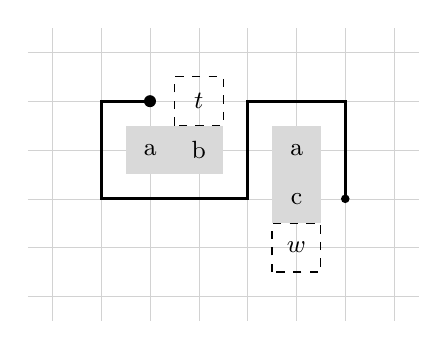
\begin{tikzpicture}[scale=0.62]
\draw[gray!35, very thin] (-2.5,-4.5) grid (5.5,1.5);
\foreach \x/\y in {0/-1, 3/-1} {\fill[gray!30] (\x-0.5,\y-0.5) rectangle (\x+0.5,\y+0.5); \node at (\x,\y) {\small a};}
\fill[gray!30] (0.5,-1.5) rectangle (1.5,-0.5); \node at (1,-1) {\small b};
\fill[gray!30] (2.5,-2.5) rectangle (3.5,-1.5); \node at (3,-2) {\small c};
\draw[dashed] (2.5,-3.5) rectangle (3.5,-2.5); \node at (3,-3) {\small $w$};
\draw[dashed] (0.5,-0.5) rectangle (1.5,0.5); \node at (1,0) {\small $t$};
\draw[very thick] (4,-2) -- (4,-1) -- (4,0) -- (3,0) -- (2,0) -- (2,-1) -- (2,-2) -- (1,-2) -- (0,-2) -- (-1,-2) -- (-1,-1) -- (-1,0) -- (0,0);
\fill (4,-2) circle (2.5pt);
\fill (0,0) circle (3.5pt);
\end{tikzpicture}
\caption{A state $S$ of $13$ cells, drawn as a path from its first cell (small dot) to the origin (large dot), entered with the last step $+e_1$, and the step $t=e_1$. Each marked cell is dead by the test of Definition~\ref{def:dead} with the same letter, test~(c) with the cell~$w$.}\label{fig:dead}
\end{figure}

\subsection{Certificates}
\begin{definition}\label{def:cert}
A \emph{certificate} of order $K$ consists of a finite set $\mathcal S$ of states that contains $S_\mathrm{st}$, an integer $V_S\ge0$ for each $S\in\mathcal S$, and, for each $S\in\mathcal S$ and each step $t$, an entry that is either the symbol $\varnothing$ or a state $S'\in\mathcal S$, such that the following hold.
\begin{enumerate}[label=(C\arabic*)]
\item If the entry for $(S,t)$ is $\varnothing$, then $t\in|S|$, or $t$ is not connected to infinity in $\Z^2\setminus|S|$.
\item If the entry for $(S,t)$ is a state $S'$ and $t\notin|S|$, then there is $g\in D_4$ such that every cell of the set $g(|S'|)+t$ lies in $E=|S|\cup\{t\}$ or is dead for $(S,t)$.
\item $V_{S_\mathrm{st}}>0$; every state with $V_S=0$ has only children with $V=0$; and there is no sequence $S_1,\dots,S_r=S_1$ ($r\ge2$) of states with $V=0$ in which each $S_{i+1}$ is a child of~$S_i$.
\end{enumerate}
Here the \emph{children} of $S$ are the states $S'$ that occur in its entries. The \emph{ratio} of the certificate is
\[
\lambda=\max\Bigl\{V_S^{-1}\sum_tV_{S'_t}:S\in\mathcal S,\ V_S>0\Bigr\},
\]
where the sum runs over the steps $t$ whose entry is a state $S'_t$.
\end{definition}

An entry $S'$ for a step $t\in|S|$ is allowed and need not satisfy any condition. Such an entry is never used by a walk and can only increase the counts below. The set $g(|S'|)+t$ in (C2) contains both $t=g(0)+t$ and the cell $g(-e_1)+t$, which is the image of the second-to-last cell of~$S'$; so (C2) requires the cell in the excluded direction $-e_1$ of the next state to lie in $E$ or to be dead. The \emph{automaton graph} of a certificate is the directed graph on $\mathcal S$ with one edge from $S$ to $S'$ for each step of $S$ whose entry is~$S'$. A \emph{path} of length $n$ in it is a sequence of $n$ edges in which each edge starts at the state where the previous one ends; states and edges may repeat.

\section{Soundness}\label{sec:sound}

\begin{theorem}\label{thm:sound}
Let a certificate of order $K$ be given. For every $n\ge1$, $b_n$ is at most the number of paths of length $n$ in the automaton graph that start at $S_\mathrm{st}$.
\end{theorem}

\begin{proof}
Fix an $n$-step bridge $\omega$ with $\omega_0=0$. For $0\le k\le n$ the \emph{past} at time $k$ is $P_k=H\cup\{\omega_0,\dots,\omega_k\}$. A cell is \emph{dead at time $k$} if no continuation of $\omega$ at time $k$ visits it after time $k$. The cells of $P_k$ are dead at time $k$, because the cells of a continuation are distinct. A cell that is dead at time $k$ is dead at every later time $j$, because a continuation at time $j$ is a continuation at time $k$, and a visit after time $j$ is a visit after time $k$.

We define states $S^k\in\mathcal S$ and isometries $\Phi_k(z)=h_k(z)+\omega_k$ of $\Z^2$, with $h_k\in D_4$, such that
\begin{equation}\label{eq:inv}
\text{every cell of }\Phi_k(|S^k|)\text{ is dead at time }k.
\end{equation}
Let $S^0=S_\mathrm{st}$ and $\Phi_0=\mathrm{id}$. Then $\Phi_0(|S^0|)\subset H\subset P_0$, so~\eqref{eq:inv} holds for $k=0$.

Suppose that $S^k$ and $\Phi_k$ satisfy~\eqref{eq:inv}, and let $k<n$. Put $t=h_k^{-1}(\omega_{k+1}-\omega_k)$, a neighbour of the origin. Let $\gamma$ be a continuation of $\omega$ at time $n$. It is also a continuation at time $k$, and it visits $\omega_{k+1}=\gamma_{k+1}$ after time $k$, so $\omega_{k+1}$ is not dead at time $k$. By~\eqref{eq:inv}, $t\notin|S^k|$. In particular $t\ne-e_1$, so $t$ is a step of $S^k$. The cells $\gamma_i$ with $i\ge k+1$ are not dead at time $k$, by the definition of dead cells, so they avoid $\Phi_k(|S^k|)$. Hence the cells $\Phi_k^{-1}(\gamma_i)$, $i\ge k+1$, form an infinite self-avoiding path that starts at $t$ and avoids $|S^k|$, and $t$ is connected to infinity in $\Z^2\setminus|S^k|$. By (C1), the entry of $(S^k,t)$ is a state $S'$. Let $g$ be the first element, in a fixed list of the elements of $D_4$, that satisfies (C2) for this entry. This choice makes the construction deterministic. Let $S^{k+1}=S'$ and $\Phi_{k+1}(z)=\Phi_k(g(z)+t)$. Then $h_{k+1}=h_kg$ and $\Phi_{k+1}(0)=\Phi_k(t)=\omega_{k+1}$.

We show~\eqref{eq:inv} for $k+1$. Let $E=|S^k|\cup\{t\}$. Every cell of $\Phi_k(E)$ is dead at time $k+1$: the cells of $\Phi_k(|S^k|)$ were dead at time $k$, and $\Phi_k(t)=\omega_{k+1}\in P_{k+1}$. Let $z$ be a cell of $g(|S'|)+t$. If $z\in E$, then $\Phi_k(z)$ is dead at time $k+1$. Otherwise $z$ is dead for $(S^k,t)$ by (C2), and we show that $\Phi_k(z)$ is dead at time $k+1$. Let $\delta$ be a continuation of $\omega$ at time $k+1$, and suppose that $\delta$ visits $\Phi_k(z)$ after time $k+1$. The cells $\delta_i$ with $i>k+1$ are not dead at time $k+1$, so they avoid $\Phi_k(E)$. Apply $\Phi_k^{-1}$, which is an isometry of $\Z^2$ that maps $\omega_{k+1}$ to $t$. The images of the cells $\delta_i$, $i>k+1$, form a self-avoiding path $\delta'$ that starts at a neighbour of $t$, avoids $E$, passes through $z$ and then goes to infinity. In case~(a), at most one neighbour of $z$ lies outside $|S^k|$. If there is none, then $\delta'$ can neither start at $z$, which is then not a neighbour of $t$, nor enter $z$. Otherwise let $u$ be this neighbour. If $z$ is the first cell of $\delta'$, then $z$ is a neighbour of $t$, so $u=t$, all four neighbours of $z$ lie in $E$, and $\delta'$ cannot leave $z$. If not, $\delta'$ enters $z$ from a neighbour outside $E$, which can only be $u$ (so $u\ne t$), and it cannot leave $z$, because the other neighbours of $z$ lie in $E$ and $\delta'$ has already visited $u$. In case~(b), $\delta'$ goes from $z$ to infinity in $\Z^2\setminus E$, which is impossible. In case~(c), let $w$ be the cell of the test and $Q$ the component of $z$ in $\Z^2\setminus(E\cup\{w\})$. The first cell of $\delta'$ is a neighbour of $t$ outside $E$, so it is not in $Q$ (it may be $w$), $Q$ is finite, and every cell adjacent to $Q$ but not in $Q$ lies in $E\cup\{w\}$. Hence $\delta'$ passes through $w$ before it reaches $z$ and again after it leaves $z$, which contradicts self-avoidance. In each case we have a contradiction, so $\Phi_k(z)$ is dead at time $k+1$. This proves~\eqref{eq:inv} for $k+1$.

Let $t_k$ be the step $t$ used at time $k$. The edges of the automaton graph given by $S^k$ and $t_k$, for $0\le k<n$, form a path of length $n$ that starts at $S_\mathrm{st}$. The bridge can be recovered from this path: $\omega_{k+1}=\Phi_k(t_k)$, and $\Phi_{k+1}$ is determined by $\Phi_k$ and by the symmetry $g$, which depends only on $S^k$, $t_k$ and the entry of $(S^k,t_k)$. Hence distinct bridges give distinct paths, which proves the theorem.
\end{proof}

\begin{remark}\label{rem:mono}
Two monotonicity facts are used in the proof. First, every cell of $\Phi_k(E)$ is dead at time $k+1$, so a continuation at time $k+1$ avoids $\Phi_k(E)$ after time $k+1$. Second, if $z$ is dead for $(S^k,t)$, then $\Phi_k(z)$ is dead at time $k+1$, although the tests (a)--(c) look only at $E$: the case analysis uses only that $\delta'$ is an infinite self-avoiding path that starts at a neighbour of $t$ and avoids $E$. The cells of the past outside $\Phi_k(E)$ play no role; self-avoidance is used at cells outside $E$ (the neighbour $u$ in case~(a), the cell $w$ in case~(c)).
\end{remark}

\section{Counting}\label{sec:count}

\begin{lemma}\label{lem:count}
Let a certificate have ratio $\lambda$, and let $L$ be the number of its states with $V=0$. The number of paths of length $n$ in the automaton graph that start at $S_\mathrm{st}$ is at most
\[
V_{S_\mathrm{st}}\,\lambda^n+3^{L+1}\,V_{S_\mathrm{st}}\sum_{k=0}^{n-1}\lambda^k.
\]
If no state has $V=0$, it is at most $V_{S_\mathrm{st}}\lambda^n$.
\end{lemma}

\begin{proof}
For $k\ge0$ and a state $S$ with $V_S>0$, let $W_k(S)$ be the number of paths of length $k$ from $S_\mathrm{st}$ to $S$ that visit only states with $V>0$. Then $\sum_SW_k(S)V_S\le\lambda^kV_{S_\mathrm{st}}$. This holds for $k=0$, and
\[
\sum_SW_{k+1}(S)V_S\le\sum_{S'}W_k(S')\sum_{t}V_{S'_t}\le\lambda\sum_{S'}W_k(S')V_{S'},
\]
where the outer sums run over states with $V>0$ and the inner sum runs over the steps $t$ of $S'$ whose entry is a state $S'_t$, as in the definition of~$\lambda$. Since $V_S\ge1$ when $V_S>0$, the number of such paths of length $k$ is at most $\lambda^kV_{S_\mathrm{st}}$. A path that leaves the states with $V>0$ does so at its first edge into a state with $V=0$, and from then on it only visits states with $V=0$, by (C3). These states form an acyclic graph with out-degrees at most $3$, so the rest of the path has length less than $L$, and there are at most $3^L$ possible rests for each first edge. The first edge into a state with $V=0$ follows a path of some length $k\le n-1$ that stays in $V>0$, and there are at most $3$ choices for it. This gives the bound.
\end{proof}

\begin{proof}[Proof of Theorem~\ref{thm:main}]
By Theorem~\ref{thm:sound} and Lemma~\ref{lem:count}, $b_n\le C\,n\max(\lambda,1)^n$ for the ratio $\lambda$ of any certificate, with $C$ independent of $n$. By~\eqref{eq:hw}, $\mu\le\max(\lambda,1)$. By the computation of Section~\ref{sec:check}, the files described there define a certificate of order $\Kmax$ in the sense of Definition~\ref{def:cert}, and its ratio $\lambda$ is the fraction in Theorem~\ref{thm:main}, which is larger than~$1$.
\end{proof}

\section{Construction of the automaton}\label{sec:build}

This section describes how we found the certificate.

Our construction program starts from the start state and explores the states reachable by steps. For a state $S$ and a step $t$ it lists several candidate children: subsets of $E=|S|\cup\{t\}$ together with dead cells, written as paths ending at $t$ and placed by a symmetry so that they end at the origin with last step $+e_1$, as in Section~\ref{sec:automata}. The size of a path $(s_0,\dots,s_{m-1})$ is $m-1+|s_{m-1}-s_0|_1$, the length of the loop obtained by closing it with a shortest lattice path. The candidates come from rules of the kind introduced by P\"onitz and Tittmann~\cite{PT00} and Couronn\'e~\cite{Cou25}:
\begin{itemize}[leftmargin=*]
\item old cells are forgotten when the size exceeds the order $K$ (Couronn\'e's parameter $k$ plays the role of $K$); at order~$\Kmax$ the size of the child that keeps all cells may exceed $K$ by a bonus of at most $8$. The bonus is read from one of two tables at the index $(m-1-|s_{m-1}-s_0|_1)/2$, which measures how far the path is from a shortest path between its ends, and a test on the shape of the child chooses the table; the README of the archive gives the tables with the build command;
\item cells cut off by bridge configurations in the sense of~\cite{Cou25}, which are not related to the bridges of Section~\ref{sec:bridges}, are recognized as dead;
\item loops sealed by the walk are treated as blocked regions;
\item steps into trapped regions get no child.
\end{itemize}

Couronn\'e also uses a rule based on the enclosure of the oldest cell of a state (Section~4.2 of the arXiv version of~\cite{Cou25}). Our section numbers and values from~\cite{Cou25} refer to this version. Our program does not use this rule, and gives a step no child only in the two cases allowed by (C1). The small-loop rule of Couronn\'e (Section~3.4 of~\cite{Cou25}) requires that neither end of a loop sealed except for one gap cell is the current position, whereas our program allows such an end to be the current position, provided that no neighbour of the current position lies inside the loop; we call this condition the guard. A variant of our program without the guard produces children that violate (C2), as the rejected certificates of Appendix~\ref{app:checks} show.

The program explores the states twice. In the second pass, when it shortens a candidate child, it may stop at any state found in the first pass. It then alternates power iteration, which gives approximate positive weights, with a new choice, for every state and step, of the candidate child of smallest weight. The weights in the certificate are those of the last power iteration, computed before the last new choice of children; that choice can only lower the sums. The ratio $\lambda$ is computed exactly from these weights.

Table~\ref{tab:ratios} compares the ratio of our certificate with the values reported in~\cite{Cou25}. It does not isolate the effect of dead cells, which would need certificates built with and without them at the same order.

\begin{table}[ht]
\caption{Upper bounds from automata: the values reported in~\cite{Cou25} and the ratio of our certificate, truncated to nine decimals and accepted by both checkers of Section~\ref{sec:check}.}\label{tab:ratios}
\centering\small
\begin{tabular}{@{}lrrr@{}}
\toprule
 & order & states & bound\\
\midrule
\cite{Cou25} & $24$ & $79{,}510{,}267$ & $2.664196283$\\
\cite{Cou25} & $26$ & $430{,}365{,}791$ & $2.662342426$\\
Theorem~\ref{thm:main} & $30$ & $\NStates$ & $2.658651241$\\
\bottomrule
\end{tabular}
\end{table}

\section{The certificate and its verification}\label{sec:check}

The checks below concern the certificate itself, so the construction of Section~\ref{sec:build} need not be trusted. The certificate for Theorem~\ref{thm:main} has order $K=\Kmax$ and $\NStates$ states, none with $V=0$. It is stored in three binary files: the states as $64$-bit keys that encode their paths, the entries as indices into the list of states, and the weights as double-precision numbers $v_S$, from which the checker computes $V_S=\lfloor2^{60}v_S\rfloor$ exactly. The README of the archive describes the format.

The checker reads the three files and verifies the following, for every state $S$ and every step $t$.
\begin{itemize}[leftmargin=*]
\item The keys are strictly increasing and decode to self-avoiding paths that end at the origin with last step $+e_1$, the start state is present, every $v_S$ lies in $[0,1]$, and every index is smaller than the number of states.
\item If the entry is $\varnothing$, then $t\in|S|$, or a flood fill from $t$ in $\Z^2\setminus|S|$ does not reach the boundary of the bounding box of $|S|$ enlarged by one cell. This is (C1).
\item If the entry is a child $S'$, the checker tries the eight symmetries $g\in D_4$ (the symmetry is not stored) and accepts the entry if for one of them every cell of $g(|S'|)+t$ lies in $E$ or passes one of the tests (a)--(c) of Definition~\ref{def:dead}. It does this also when $t\in|S|$, where Definition~\ref{def:cert} requires nothing. For (b) it uses a flood fill in $\Z^2\setminus E$ to the boundary of the bounding box of $E$ enlarged by one cell. For (c) it tries as $w$ the cells of one shortest path in $\Z^2\setminus E$ from $z$ to that boundary; since (b) has failed, such a path exists. A cell outside the bounding box of $E$ stays connected to infinity when any one other cell is removed, so a flood fill with $w$ removed decides whether $z$ is connected to infinity in $\Z^2\setminus(E\cup\{w\})$. Every cell $w$ for which (c) holds lies on every path from $z$ to the boundary, in particular on the chosen one. This is (C2).
\item It computes the ratio $\lambda$ as an exact fraction in integer arithmetic and checks (C3).
\end{itemize}
The checker accepts the certificate, and its ratio is the fraction of Theorem~\ref{thm:main}.

A second, independently written checker also accepts the certificate, with the same ratio; Appendix~\ref{app:checks} describes it and the tests of both checkers.


\section{Formal verification}\label{sec:lean}

Using the Lean~4 proof assistant \cite{Lean4} and the Mathlib library \cite{Mathlib}, we also proved Theorem~\ref{thm:main}, with the certificate of Section~\ref{sec:check}. The formal theorem has no hypotheses:
\begingroup\footnotesize
\begin{verbatim}
theorem connective_constant_le_unconditional :
    ∃ μ : ℝ, Tendsto (fun n : ℕ => (sawCount n : ℝ) ^ ((1 : ℝ) / n)) atTop (𝓝 μ) ∧
      μ ≤ (105432502045487 : ℝ) / 39656386815908 ∧ μ < 2.6586513
\end{verbatim}
\endgroup
\noindent It states that $c_n^{1/n}$ converges to a limit $\mu$, that $\mu\le\LamRedNum/\LamRedDen$ and that $\mu<\MuUB$. Here \lean{sawCount n} is $c_n$: a walk is given by its sequence of $n$ steps in $\{e_1,-e_1,e_2,-e_2\}$, its $n+1$ points are the partial sums of its steps, the first being the origin, and \lean{sawCount n} is the number of step sequences whose points are distinct.
\begingroup\footnotesize
\begin{verbatim}
def walk {n : ℕ} (s : Fin n → Fin 4) (i : Fin (n + 1)) : Cell :=
  ∑ j : Fin n, if (j : ℕ) < (i : ℕ) then dir (s j) else 0

def sawCount (n : ℕ) : ℕ :=
  (univ.filter fun s : Fin n → Fin 4 => Function.Injective (walk s)).card
\end{verbatim}
\endgroup
\noindent Here \lean{Cell} is $\Z\times\Z$ and \lean{dir} maps $0,1,2,3$ to $e_1,-e_1,e_2,-e_2$. Apart from \lean{Cell}, \lean{dir}, \lean{walk} and \lean{sawCount}, the statement uses only definitions from Lean's core library and from Mathlib.

The formal proof follows the paper. Its definition of a certificate is Definition~\ref{def:cert} with (C3) replaced by the condition $V_S>0$ for all $S$; for such certificates it contains Theorem~\ref{thm:sound} and Lemma~\ref{lem:count}. It also contains the submultiplicativity $c_{m+n}\le c_mc_n$ and the existence of $\mu$ by Fekete's lemma. In the proof of Theorem~\ref{thm:sound} it uses one continuation $\gamma$ of the bridge, the one through the history, the bridge and its translates (Section~\ref{sec:bridges}). It replaces~\eqref{eq:inv} by the statement that $\gamma$ does not visit $\Phi_k(|S^k|)$ after time $k$, proved by the case analysis above, and~\eqref{eq:hw} by a weaker form of the Hammersley--Welsh inequality,
\begin{equation}\label{eq:hwweak}
c_n\le(n+1)^{2\lfloor\sqrt{2n}\rfloor+1}\,b_{n+1},
\end{equation}
which suffices because the factor is $e^{o(n)}$. The proof splits the walk at the first time at which its first coordinate is smallest and unfolds each of the two parts by reflections. The injection records the split time and the times of the at most $\lfloor\sqrt{2n}\rfloor$ reflections in each part. With a step $e_1$ put in front, this gives an injective map from walks to pairs of such a record and a bridge of $n+1$ steps, and there are at most $(n+1)^{2\lfloor\sqrt{2n}\rfloor+1}$ records. With the bound for $b_n$, this inequality yields $\mu\le\lambda$.

The certificate is checked by a program written in Lean, and a Lean proof shows that every certificate it accepts satisfies the formal definition with ratio at most $\lambda$. In this first formal proof, the check runs as compiled code, split into theorems proved by \lean{native_decide}, so its trusted base includes the Lean compiler and interpreter, the C compiler that Lean uses and the Lean runtime. Besides the standard axioms \lean{propext}, \lean{Classical.choice} and \lean{Quot.sound}, the theorem depends on one auxiliary axiom for each compiled check, and the rest of the proof, including the soundness of the checking program and inequality~\eqref{eq:hwweak}, is checked by Lean's kernel.

A second formal proof of Theorem~\ref{thm:main}, with the same statement, is in the directory \texttt{\KDir/} of the archive. Since it depends only on \lean{propext}, \lean{Classical.choice} and \lean{Quot.sound}, it needs no code generated by Lean's compiler, and its trusted base is Lean's kernel, including the kernel's built-in arithmetic on natural numbers. A proof of this kind for the weaker bound $\mu<2.6614721$, from an earlier certificate of order~$26$, is archived at \href{https://doi.org/\VsixSuppDOI}{doi:\VsixSuppDOI}. Appendix~\ref{app:checks} describes both checks.

\section{Concluding remarks}\label{sec:end}

The bound of Theorem~\ref{thm:main} remains about $0.02$ above the numerical estimate of~\cite{JSG16}. In~\cite{Cou25}, raising the order from $24$ to $26$ lowers the bound by about $0.002$ and multiplies the number of states by about $5.4$, and our automaton of order~$\Kmax$ already has about $2.5\cdot10^{10}$ states, for which the first checker of Section~\ref{sec:check} needs about $1.3$ terabytes of memory. The method is thus limited by the size of the automaton. Lowering the bound further at a manageable size therefore needs rules or tests that lower the ratio at a given order, for instance tests that recognize more dead cells.

\appendix
\section{Details of the checks}\label{app:checks}

\subsection{The second checker and the tests}
The checking logic of the second checker of Section~\ref{sec:check} was first written from the description of the checked conditions, before its author read the first checker; the version used differs from this first version only in its output and in three changes that can only cause a rejection, which the README of its directory lists. It uses flood fills on rows stored as bit masks, and for (c) it tries as $w$ only the cells of the component of $z$ in $\Z^2\setminus E$ that share a side or a corner with a cell of $E$. No valid $w$ is missed. Test (b) has shown that $z$ is connected to infinity, and removing a cell $w$ leaves $z$ connected to infinity in two cases: if none of the eight cells around $w$ lies in $E$, because these cells then connect the four neighbours of $w$; and if $w$ lies outside the component of $z$, because removing $w$ then does not change that component. The two checkers report the same numbers of entries $\varnothing$, of entries with a child and of dead cells of each kind, although they list $D_4$ in different orders, on which the counts of dead cells depend.

A program in Python also checks certificates of order $10$, $12$ and $14$. They were built by the same construction program with the same rules and the default values of its other parameters, without the tables of bonuses used at order~$\Kmax$. Unlike the two checkers, it tries as $w$ every cell of the bounding box of $E$ enlarged by one cell, and it gives the same ratios as the two checkers. Both checkers accept the certificates of order $10$ to $16$ built in this way.

Both checkers reject certificates that must fail (those of orders $12$, $14$ and $16$ built without the guard of Section~\ref{sec:build}, and the accepted certificate of order $16$ with a child removed or children redirected), and both report a larger ratio after a weight of that certificate is halved.

\subsection{The formal proofs}
The checking program of the first formal proof checks the conditions of Definition~\ref{def:cert} for every state, with positive weights and the ratio of Theorem~\ref{thm:main}. Every claim that a cell is not connected to infinity, or in test~(c) to a neighbour of $t$, is checked again on the region that the flood fill returns: this region must contain the cell and lie in a bounded box, every unblocked neighbour of its cells must lie in it, and in test~(c) it must contain no unblocked neighbour of $t$; so errors in the flood fills or in the search for $w$ cannot lead to an acceptance. Neither the construction of the automaton (Section~\ref{sec:build}) nor the largest ratio is computed in Lean; the program checks only that $V_S^{-1}\sum_tV_{S'_t}\le\lambda$ for every state $S$.

The certificate enters as data, converted into records that Lean compiles into string constants; the checking program checks whatever records it is given, and the theorem follows if the check succeeds.

The general parts of the proof (the soundness of the checking program, the cover of the states by the compiled checks, Theorem~\ref{thm:sound}, Lemma~\ref{lem:count}, the bound $\mu\le\lambda$ from the bound for $b_n$, and inequality~\eqref{eq:hwweak}) depend only on the standard axioms.

The second formal proof checks the certificate inside Lean's kernel. Instead of trying the eight symmetries for a child and the three tests for a dead cell, its checking program reads hints: the symmetry to use, and the test (a), (b) or (c) that applies, with the cell $w$ for test~(c). The hints are computed beforehand by compiled code but are not trusted, since a wrong hint can only make the check fail; the README of the directory \texttt{\KDir/} describes the structure of this proof and its build. For both formal proofs, the general parts were also accepted by two further implementations of the Lean kernel, nanoda~\cite{nanoda} and lean4lean~\cite{Car24}.

\section*{Data availability}
\begingroup\sloppy
The two checkers, the program in Python, the construction program, the programs for the tests of Appendix~\ref{app:checks}, and the Lean files of both formal proofs of Section~\ref{sec:lean} with the programs that generate their data files are archived at \href{https://doi.org/\SUPPDOI}{doi:\SUPPDOI}, together with the list of the units of the second formal proof, the SHA-256 checksums of their compiled files, and the compiled public files of its data modules, part modules and root. The three files of the certificate were compressed with xz, the file of entries in four pieces and the file of weights in five; the ten compressed files are archived in five records, \href{https://doi.org/\DataA}{doi:\DataA}, \href{https://doi.org/\DataB}{doi:\DataB}, \href{https://doi.org/\DataC}{doi:\DataC}, \href{https://doi.org/\DataD}{doi:\DataD} and \href{https://doi.org/\DataE}{doi:\DataE}.

Three earlier certificates of ours, of orders $26$ and $28$, built by an earlier version of the construction program, are also archived, and both checkers accept them. The one of order~$28$ with $5{,}792{,}114{,}594$ states is at \href{https://doi.org/\FSuppDOI}{doi:\FSuppDOI} (keys and weights) and at \href{https://doi.org/\FDataDOI}{doi:\FDataDOI} (entries). The other two are at \href{https://doi.org/\OldSuppDOI}{doi:\OldSuppDOI}; they have fewer than $2^{32}-1$ states and store the entries as $32$-bit indices, with $2^{32}-1$ for $\varnothing$. The second checker uses $32$-bit indices exactly when there are fewer than $2^{32}-1$ states. The first checker takes the width from the size of the file of entries. The repository \url{\REPOURL}\COMMITREF{} also holds the programs and the Lean files.\par\endgroup

\section*{Use of AI tools}
Generative AI tools were used to find and prove the results, to write the programs and the Lean formalization, and to draft the text. The author reviewed the arguments, the programs and the formal statements, and takes responsibility for the content.

\begin{thebibliography}{99}
\bibitem{Alm93} S.~E.~Alm, \emph{Upper bounds for the connective constant of self-avoiding walks}, Combin. Probab. Comput. \textbf{2} (1993), 115--136.
\bibitem{Car24} M.~Carneiro, \emph{Lean4Lean: verifying a typechecker for Lean, in Lean}, arXiv:2403.14064, 2024.
\bibitem{Cou25} O.~Couronn\'e, \emph{New upper bound for the connective constant for square-lattice self-avoiding walks}, J. Stat. Phys. \textbf{192} (2025), 153; arXiv:2211.16146.
\bibitem{DCS12} H.~Duminil-Copin and S.~Smirnov, \emph{The connective constant of the honeycomb lattice equals $\sqrt{2+\sqrt2}$}, Ann. of Math. (2) \textbf{175} (2012), 1653--1665.
\bibitem{HaMo54} J.~M.~Hammersley and K.~W.~Morton, \emph{Poor man's Monte Carlo}, J. Roy. Statist. Soc. Ser. B \textbf{16} (1954), 23--38.
\bibitem{HW62} J.~M.~Hammersley and D.~J.~A.~Welsh, \emph{Further results on the rate of convergence to the connective constant of the hypercubical lattice}, Quart. J. Math. Oxford Ser. (2) \textbf{13} (1962), 108--110.
\bibitem{JSG16} J.~L.~Jacobsen, C.~R.~Scullard and A.~J.~Guttmann, \emph{On the growth constant for square-lattice self-avoiding walks}, J. Phys. A \textbf{49} (2016), 494004.
\bibitem{Jen04} I.~Jensen, \emph{Improved lower bounds on the connective constants for two-dimensional self-avoiding walks}, J. Phys. A \textbf{37} (2004), 11521--11529.
\bibitem{MS93} N.~Madras and G.~Slade, \emph{The Self-Avoiding Walk}, Birkh\"auser, Boston, 1993.
\bibitem{Mathlib} The mathlib Community, \emph{The Lean mathematical library}, in: Proc. 9th ACM SIGPLAN Int. Conf. Certified Programs and Proofs (CPP 2020), 2020, 367--381.
\bibitem{Lean4} L.~de~Moura and S.~Ullrich, \emph{The Lean 4 theorem prover and programming language}, in: Automated Deduction -- CADE 28, Lecture Notes in Comput. Sci. \textbf{12699}, Springer, 2021, 625--635.
\bibitem{nanoda} \lean{nanoda_lib}, a type checker for Lean~4, \url{https://github.com/ammkrn/nanoda_lib}.
\bibitem{Noo98} J.~Noonan, \emph{New upper bounds for the connective constants of self-avoiding walks}, J. Stat. Phys. \textbf{91} (1998), 871--888.
\bibitem{PT00} A.~P\"onitz and P.~Tittmann, \emph{Improved upper bounds for self-avoiding walks in $\Z^d$}, Electron. J. Combin. \textbf{7} (2000), R21.
\end{thebibliography}

\end{document}
